%! TeX program = lualatex
\documentclass[../main.tex]{subfiles}
\begin{document}
Optimization is a landmark application of differential calculus.  
To optimize something means to find the largest/smallest, most/least, etc. of something. 

Sections 4.3 (Extrema), 4.5 (Derivative Tests) and 4.7 (Optimization) are all connected.

\faExclamationTriangle{} There are almost no routine problems in optimization. But every question is very doable. Suggested problems in Sections 4.3, 4.5 and 4.7 offer excellent opportunities to improve our problem-solving skills.

\begin{lesson}{Maxima and Minima}
  % Finding absolute extrema is very useful for \sout{science} just about everything. The idea: It is straightforward to find the max (or min) of \hlmain{a \emph{finite} list of values}. To find absolute extrema of a function, it would be nice if we can \hlmain{narrow} the search for absolute extrema from \emph{infinitely} many numbers on the domain to \hlsupp{a handful of candidates} on the domain and compare their values manually. But we have to be mindful of the big picture to fully understand the subtle details.

  \begin{example} \label{ex:abs-extrema}
    For each function below, identify \emph{all} of its absolute maximum and absolute minimum on the given interval or explain why no absolute extremum exists on the given interval.

    \begin{center}
      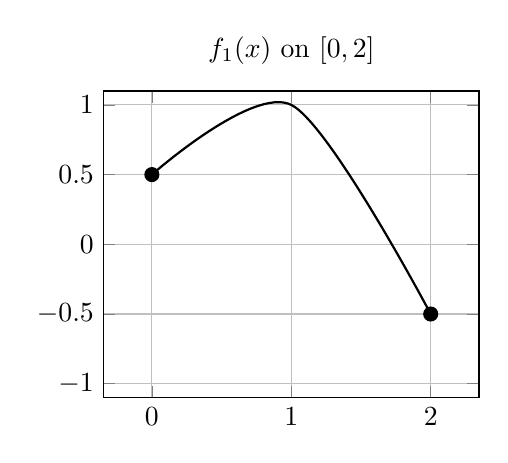
\begin{tikzpicture}[scale=1]
        \begin{axis}[width=2.5in, axis equal, xmin=0, xmax=2, ymin=-1, ymax=1, enlargelimits=0.05, title={\(f_{1}(x)\) on \([0,2]\)}, grid=major, ylabel={}]
          \addplot[thick, smooth] coordinates {(0,1/2) (1,1) (2,-1/2)};
          \draw[fill=black] (axis cs:0,1/2) circle[radius=0.05];
          \draw[fill=black] (axis cs:2,-1/2) circle[radius=0.05];
        \end{axis}
      \end{tikzpicture}
      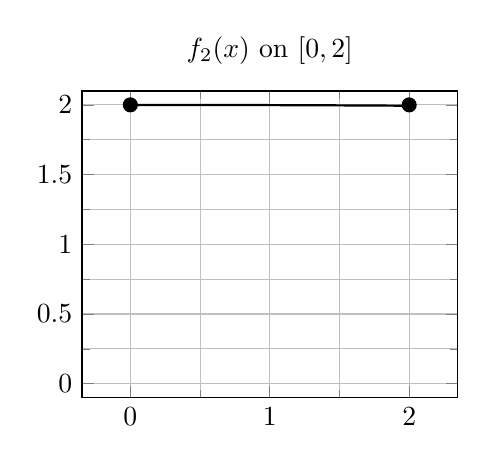
\begin{tikzpicture}[scale=1]
        \begin{axis}[width=2.5in, axis equal, xmin=0, xmax=2, ymin=0, ymax=2, enlargelimits=0.05, title={\(f_{2}(x)\) on \([0,2]\)}, grid=both, minor tick num=1, ylabel={}]
          \addplot[thick, domain=0:2, smooth, samples=100] { cos(pi*x) + 1};
          \draw[fill=black] (axis cs:0,2) circle[radius=0.05];
          \draw[fill=black] (axis cs:2,2) circle[radius=0.05];
        \end{axis}
      \end{tikzpicture}
      \begin{tikzpicture}[scale=1]
        \begin{axis}[width=2.5in, axis equal, xmin=-1, xmax=1, ymin=0, ymax=2, enlargelimits=0.05, title={\(f_{3}(x) = \tfrac{1}{x^{2}+1}\) on \((-\infty, \infty)\)}, xtick={-1,0,1}, xticklabels={-10,0,10}, grid=major, ylabel={}]
          \addplot[thick, smooth, samples=100] {1/((sqrt(10)*x)^2+1)};
        \end{axis}
      \end{tikzpicture}
    \end{center}
    \vfill{}

    \begin{center}
      \begin{tikzpicture}[scale=1]
        \begin{axis}[width=2.5in, axis equal, xmin=0, xmax=2, ymin=-2, ymax=0, enlargelimits=0.05, title={\(f_{4}(x)\) on \((0,2)\)}, grid=major, ylabel={}]
          \addplot[thick, domain=0:2, smooth, samples=100] {(1/5)*(x-1)/(x*(2-x))-1};
        \end{axis}
      \end{tikzpicture}
      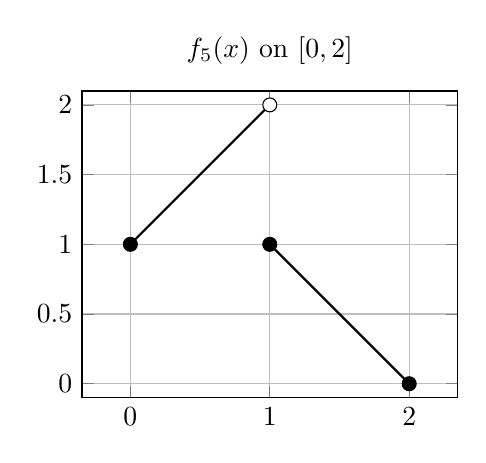
\begin{tikzpicture}[scale=1]
        \begin{axis}[width=2.5in, axis equal, xmin=0, xmax=2, ymin=0, ymax=2, enlargelimits=0.05, title={\(f_{5}(x)\) on \([0,2]\)}, grid=major, ylabel={}]
          \addplot[thick] coordinates {(0,1) (1,2)};
          \addplot[thick] coordinates {(1,1) (2,0)};
          \draw[fill=black] (axis cs:0,1) circle[radius=0.05];
          \draw[fill=white] (axis cs:1,2) circle[radius=0.05];
          \draw[fill=black] (axis cs:1,1) circle[radius=0.05];
          \draw[fill=black] (axis cs:2,0) circle[radius=0.05];
        \end{axis}
      \end{tikzpicture}
      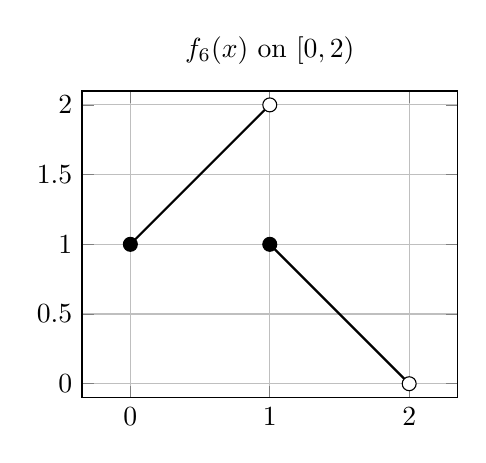
\begin{tikzpicture}[scale=1]
        \begin{axis}[width=2.5in, axis equal, xmin=0, xmax=2, ymin=0, ymax=2, enlargelimits=0.05, title={\(f_{6}(x)\) on \([0,2)\)}, grid=major, ylabel={}]
          \addplot[thick] coordinates {(0,1) (1,2)};
          \addplot[thick] coordinates {(1,1) (2,0)};
          \draw[fill=black] (axis cs:0,1) circle[radius=0.05];
          \draw[fill=white] (axis cs:1,2) circle[radius=0.05];
          \draw[fill=black] (axis cs:1,1) circle[radius=0.05];
          \draw[fill=white] (axis cs:2,0) circle[radius=0.05];
        \end{axis}
      \end{tikzpicture}
    \end{center}
  \end{example}

  \begin{mdframed}[style=withref-compact]
    Let \(f\) be a function defined over an interval \(I\) and let \(c \in I\).  We say
    \begin{itemize}
      \item \(f\) has an \hlmain{absolute maximum on \(I\) at \(c\)} if \underline{\hspace{2.5in}}.

      \item \(f\) has an \hlmain{absolute minimum on \(I\) at \(c\)} if \underline{\hspace{2.5in}}.

      \item If \(f\) has an absolute maximum on \(I\) at \(c\) or an absolute minimum on \(I\) at \(c\), we say \(f\) has an \hlmain{absolute extremum} on \(I\) at \(c\).
    \end{itemize}
    \textbook{Definition on page 366}
  \end{mdframed}

  The plural of maxim\hlmain{um} is maxim\hlsupp{a}, minim\hlmain{um} is minim\hlsupp{a}, and extrem\hlmain{um} is extrem\hlsupp{a}.  Some textbooks use \emph{global} instead of \emph{absolute}. For example, global maximum and absolute maximum have exactly the same meaning.

  \faExclamationTriangle{} The \hlsupp{absolute} in absolute extrema should be interpreted as ``\hlsupp{for certain}'' and has nothing do with taking absolute values.
  \clearpage

  From Example~\ref{ex:abs-extrema}, we might \hlwarn{guess} that absolute maxima and absolute minima either occur at an endpoint or wherever horizontal tangent lines show up.

  Close! But not quite. \url{https://www.geogebra.org/calculator/v98xbhbt} (the graph in Example~\ref{ex:critical-numbers}).

  \begin{mdframed}[style=withref-compact]
    Let \(f\) be a function defined over an interval \(I\).

    \begin{itemize}[noitemsep]
      \item \(f\) has a \hlmain{local maximum at \(c\)} if \(f(c) \ge f(x)\) for every \(x\) \hlmain{near} \(c\) but \(x\) cannot be an endpoint of \(I\).
      \item \(f\) has a \hlmain{local maximum at \(c\)} if \(f(c) \le f(x)\) for every \(x\) \hlmain{near} \(c\) but \(x\) cannot be an endpoint of \(I\).
      \item \(f\) has a \hlmain{local extremum at \(c\)} if \(f\) has a local maximum or local minimum at \(c\).
    \end{itemize}

    \textbook{Definition on page 368, slightly simplified}
  \end{mdframed}
  \faExclamationTriangle{} Notice the definition does not allow local extrema to occur at an endpoint of the domain of \(f\).

  \begin{mdframed}[style=withref-compact]
    Let \(f(x)\) be a function. A \hlmain{critical number} \(c\) is a constant in the domain of \(f\) (but NOT an endpoint) if 
    \[
      f'(c) = 0 \text{ or } f'(c) \text{ does not exist}.
    \]
    If \hlmain{\(c\) is a critical number} of \(f(x)\), then \hlsupp{\((c, f(c))\)} is called a \hlsupp{critical point}.

    \textbook{Definition on page 369}
  \end{mdframed}

  \begin{center}
    \begin{tabular}{c|l|l}
      Domain of \(f\) & Where to find critical numbers? & Critical number cannot be \ldots{} \\\midrule
      \([a,b]\) or \((a,b]\) or \([a,b)\) or \((a,b)\) & & \\[1ex]\midrule
      \((-\infty, b]\) & & \\[1ex]\midrule
      \([a, \infty)\) & & \\[1ex]\midrule
    \end{tabular}
  \end{center}
  
  \begin{example} \label{ex:critical-numbers}
    Consider \(f(x)\) whose graph is given below. Find all critical numbers of \(f(x)\) and identify its absolute extrema.

    \begin{center}
      \includegraphics[height=3in]{../standalones/build/extrema_example_blank.pdf}
    \end{center}
  \end{example}
  \clearpage

  \begin{example} \label{ex:critical-number-polynomial}
    Find critical numbers of \(f(x) = \frac{x^{3}}{3} - \frac{3}{2}x^{2} + 2x\) over \([0, 5/2]\).
    \blanklines{15}
  \end{example}

  \begin{example} \label{ex:critical-number-trig}
    Find critical numbers of \(f(x) = \cos(x)\) on \([0, 2\pi]\).

    \blanklines{10}
  \end{example}

  \begin{example} \label{ex:critical-number-rational}
    Find critical numbers of \(f(x) = \frac{3}{2} x^{2/3} - \frac{x^{2}}{2}\) over \([-2,2]\). 

    \blanklines{20}
  \end{example}
  \clearpage

  \begin{example} \label{ex:critical-number-is-candidate}
    If \(c\) is a critical number, is it true that \(f(c)\) is a local extrema?

    \begin{center}
      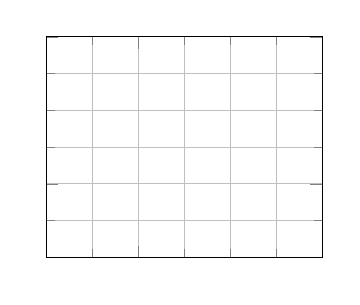
\begin{tikzpicture}[scale=1]
        \begin{axis}[xmin=-1/2, xmax=1, ymin=-1/2, ymax=1, width=2in, xtick={-1,0,1},ytick={-1,0,1},xticklabels={},yticklabels={},grid=both,minor tick num=3]
        \end{axis}
      \end{tikzpicture}
      \quad
      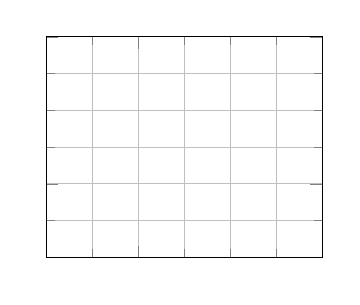
\begin{tikzpicture}[scale=1]
        \begin{axis}[xmin=-1/2, xmax=1, ymin=-1/2, ymax=1, width=2in, xtick={-1,0,1},ytick={-1,0,1},xticklabels={},yticklabels={},grid=both,minor tick num=3]
        \end{axis}
      \end{tikzpicture}
      \quad
      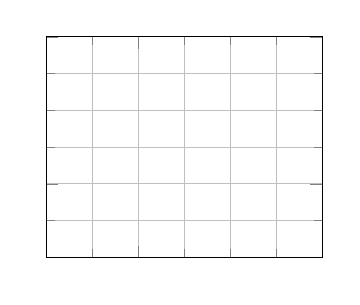
\begin{tikzpicture}[scale=1]
        \begin{axis}[xmin=-1/2, xmax=1, ymin=-1/2, ymax=1, width=2in, xtick={-1,0,1},ytick={-1,0,1},xticklabels={},yticklabels={},grid=both,minor tick num=3]
        \end{axis}
      \end{tikzpicture}
      \quad
      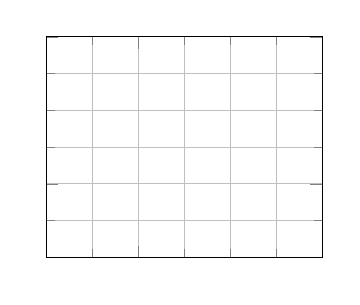
\begin{tikzpicture}[scale=1]
        \begin{axis}[xmin=-1/2, xmax=1, ymin=-1/2, ymax=1, width=2in, xtick={-1,0,1},ytick={-1,0,1},xticklabels={},yticklabels={},grid=both,minor tick num=3]
        \end{axis}
      \end{tikzpicture}
    \end{center}
  \end{example}

  Fermat's Theorem (read Theorem 4.2 on page 369) says that if \(f\) has a local extremum at \(c\) and \(f'(c)\) exists, then \(f'(c) = 0\). Together with the definition of local extrema, we immediately get the following general strategy.

  \begin{mdframed}[style=simple-compact]
    \textbf{General strategy for finding absolute extrema}. 

    If \(f\) has an \hlattn{absolute extrema} over an interval \(I\) at \(c\), then there are only \hlattn{two possibilities}:
    \begin{enumerate}
      \item Either \(c\) is \underline{\hspace{4in}},
      \item or \(c\) is \underline{\hspace{4in}}.
    \end{enumerate}
  \end{mdframed}

  Suppose we want to find absolute maxima and absolute minima of a function \(f(x)\) over an interval \(I\).
  \begin{enumerate}
    \item If \(I = [a,b]\) (closed and bounded), then compare values of \(f(a), f(b)\) and \(f(c)\) for all critical numbers \(c\).

    \item Attempt to \hlmain{rule out} the non-existence of absolute extrema by checking \(\lim_{x \to c}f(x)\) where \(c\) is any asymptote in \(I\) or any open endpoint of \(I\).
      \begin{enumerate}
        \item If we can \hlmain{rule out the non-existence} of absolute maxima, then compare values of \(f(c)\) for all critical numbers \(c\).
        \item If we can \hlmain{rule out the non-existence} of absolute minima, then compare values of \(f(c)\) for all critical numbers \(c\).
      \end{enumerate}
  \end{enumerate}
  \bigskip{}

  \faExclamationTriangle{} The definitions of local extrema and critical numbers vary from textbook to textbook. Some textbooks (e.g. UBC's CLP Calculus) allow endpoints to be local extrema, \hlwarn{For grading purposes, \thecoursesubj{}~\thecoursenumb{} will stick to the course textbook's definition} that local extrema and critical numbers cannot occur at endpoints of the domain of \(f\).


  \medskip{}
  Here is one last theoretical statement, and then we will move on to examples. 

  \begin{mdframed}[style=withref-compact]
    If \(f(x)\) is continuous over a closed and bounded interval \([a,b]\), then \(f\) must have an absolute maximum \hlsupp{and} an absolute minimum on \([a,b]\).

    \textbook{Theorem 4.1 Extreme Value Theorem on page 367}
  \end{mdframed}
  We are not required to know the proof of Extreme Value Theorem, and it says something very simple: The Extreme Value Theorem guarantees that a continuous functions defined on a closed and bounded interval always have both absolute extrema.
  \clearpage

  \begin{example} \label{ex:closed-interval-method-intro}
    Find the absolute maximum and the absolute minimum of \(f(x) = \frac{x^{3}}{3} - \frac{3}{2}x^{2} + 2x\) over \([0,5/2]\) and state wherever those values occur. Note \(f(5/2) = 5/6\).

    This is the function from Example~\ref{ex:critical-number-polynomial}. Graph: \url{https://www.geogebra.org/calculator/knx2tzaa}

    \blanklines{20}
  \end{example}

  \begin{example} 
    Find the absolute maximum and absolute minimum of \(f(x) = \frac{3}{2} x^{2/3} - x^{2}/2\) over \([-2,2]\) and state where those values occur.

    This is the function from Example~\ref{ex:critical-number-rational}. Graph: \url{https://www.geogebra.org/calculator/auvadcuj}

    \blanklines{20}
  \end{example}
  \clearpage

  \begin{example} \label{ex:extremum-open-interval}
    Find the absolute maximum and the absolute minimum of \(f(x) = \frac{1}{x^{2}+1}\) on its domain or explain why one or both of them do not exist. If an absolute extremum exist, also state where such value occur.

    Graph: \url{https://www.geogebra.org/calculator/ctet6nnb}

    \blanklines{40}
  \end{example}
\end{lesson}
\end{document}
